\documentclass[11pt,a4paper]{article}

\usepackage[margin=2.5cm]{geometry}
\usepackage{amsmath, amssymb, amsthm}
\usepackage[english, greek]{babel}
\usepackage{fontspec}
\setmainfont{DejaVu Serif}
\usepackage{microtype}
\usepackage{xcolor}

\usepackage{pgfplots}
\usepackage{tikz}
\usetikzlibrary{decorations.pathreplacing, calc}
\pgfplotsset{compat=1.18}

\title{\textbf{\Huge Jump Mechanics Notes}}
\author{\Large Nikolas Menychtas}
\date{\today}

\begin{document}

\maketitle
\hrule
\vspace{15pt}

\section{Jump Mechanics}

Αρχικά θα ορίσουμε τον \foreignlanguage{english}{player} ως ένα σημείο, αγνοούμε τις διαστάσεις του, τη μάζα του κλπ. Ακόμα θα θεωρήσουμε ότι η μόνη εξωτερική δύναμη που δέχεται ο \foreignlanguage{english}{player} είναι η δύναμη της βαρύτητας αγνοώντας την αντίσταση του αέρα.

\vspace{5pt}
Η βαρύτητα \foreignlanguage{english}{g} προκαλεί σταθερή επιτάχυνση καθόλη τη διάρκεια του χρόνου. \textbf{ΔΕΝ ΑΛΛΑΖΕΙ} με το ύψος ούτε με τον χρόνο.

\bigskip
\textbf{Όροι λογισμού / φυσικής:}
\begin{align*}
f(t) &: \text{η θέση του παίχτη στη δεδομένη στιγμή } t \\
f'(t) &: \text{η ταχύτητα του παίχτη στη δεδομένη στιγμή } t \\
f''(t) &: \text{η επιτάχυνση του παίχτη στη δεδομένη στιγμή } t
\end{align*}
\vspace{5pt}

\subsection*{Γράφημα Επιτάχυνσης}

\begin{center}
\begin{tikzpicture}
    \begin{axis}[
        axis lines = middle,
        xlabel = {$t$ (χρόνος)},
        ylabel = {$f''(t)$ (επιτάχυνση)},
        xtick=\empty,
        ytick=\empty,
        xmin=-0.5, xmax=5,
        ymin=-6, ymax=4,
        every axis x label/.style={at={(current axis.right of origin)},anchor=north west},
        every axis y label/.style={at={(current axis.above origin)},anchor=south east}
    ]
        \addplot[blue, ultra thick] coordinates {(-0.5,-3) (4.5,-3)};
        \node[above, fill=white, inner sep=2pt] at (axis cs:2.5,-3) {$f''(t) = g < 0$};
    \end{axis}
\end{tikzpicture}
\end{center}

Η $g$ προκαλεί "τράβηγμα" προς τα κάτω και η $g$ είναι σταθερή σε κάθε $t$.

\bigskip
Αν τώρα ολοκληρώσουμε την επιτάχυνση, δηλαδή την $f''(t)=g$, "ανεβαίνουμε" ένα επίπεδο και πάμε στην $f'(t)$, δηλαδή στην ταχύτητα/velocity.

\bigskip
\textbf{Άρα έχουμε:}

\begin{align}
    \int f''(t) \, dt &= \int g \, dt \notag \\
    u(t) &= g \cdot t + C \label{eq:velocity}
\end{align}

\vspace{5pt}
Για να βρούμε τη σταθερά $C$, χρησιμοποιούμε την αρχική συνθήκη.
Ξεκινάμε από τη χρονική στιγμή $t_0 = 0$, όπου η ταχύτητα είναι η αρχική ταχύτητα ($u_0$ ή $v_0$):

\begin{align}
    u(0) &= g \cdot 0 + C \notag \\
    u(0) &= C \implies C = v_0 \label{eq:constant_c}
\end{align}

Επομένως, συνδυάζοντας τις σχέσεις \eqref{eq:velocity} και \eqref{eq:constant_c}, τελικά έχουμε:
\begin{equation*}
    u(t) = g \cdot t + v_0
\end{equation*}

\subsection*{Γράφημα Ταχύτητας}

\begin{center}
\begin{tikzpicture}
    \begin{axis}[
        axis lines = middle,
        xlabel = {$t$ (χρόνος)},
        ylabel = {$f'(t)$ (ταχύτητα)},
        xtick=\empty,
        ytick=\empty,
        xmin=-0.5, xmax=6.5,
        ymin=-5, ymax=8,
        every axis x label/.style={at={(current axis.right of origin)},anchor=north west},
        every axis y label/.style={at={(current axis.above origin)},anchor=south east}
    ]
        \addplot[blue, thick, domain=0:4] {-3*x+6};
        \node[above left] at (axis cs:4.5,-3) {$f'(t) = g\cdot t +v_0$};
        \node[left] at (axis cs:0,6) {$v_0$};
    \end{axis}
\end{tikzpicture}
\end{center}

Για να βρούμε τώρα την $f(t)$ δηλαδή το position, ολοκληρώνουμε την $f'(t)$.
Άρα:
\begin{align}
    \int f'(t)\cdot dt &= \int (g \cdot t +v_0)\cdot dt \notag \\
    \iff f(t) &= \frac{1}{2}\cdot g\cdot t^2 + v_0\cdot t + C \label{eq:position}
\end{align}

\vspace{5pt}
Για να βρούμε τη σταθερά $C$, χρησιμοποιούμε την αρχική συνθήκη.
Ξεκινάμε από τη χρονική στιγμή $t_0 = 0$:
\begin{align}
    f(0) = \frac{1}{2}\cdot g \cdot 0^2 + v_0 \cdot 0 + C \iff f(0) = C_2 \label{eq:constant_c_2}
\end{align}
Συμβολίζουμε το $C_2$ ως $p_0$.

Επομένως, συνδυάζοντας τις σχέσεις \eqref{eq:position} και \eqref{eq:constant_c_2}, τελικά έχουμε:
\begin{equation*}
    f(t) = \frac{1}{2}\cdot g \cdot t^2 + v_0 \cdot t + p_0 
\end{equation*}

\begin{center}
\begin{tikzpicture}
    \begin{axis}[
        axis lines = middle,
        xlabel = {$t$ (χρόνος)},
        ylabel = {$f(t)$ (θέση)},
        xtick=\empty,
        ytick=\empty,
        xmin=-0.5, xmax=6.5,
        ymin=-2, ymax=8,
        every axis x label/.style={at={(current axis.right of origin)},anchor=north west},
        every axis y label/.style={at={(current axis.above origin)},anchor=south east}
    ]
        \addplot[blue, thick, domain=0:4] {-1.5*x^2 + 6*x + 0};
        \node[above right] at (axis cs:3.5,2) {$f(t) = \frac{1}{2}\cdot g\cdot t^2 +v\cdot t + p_0$};
    \end{axis}
\end{tikzpicture}
\end{center}

\bigskip
\textbf{Ιδιότητες Παραβολής:}
\begin{enumerate}
    \item Είναι \textbf{ΠΑΝΤΑ} συμμετρική.
    \item Το πόσο ανοιχτή ή κλειστή είναι η καμπύλη έχει να κάνει με το $a=\frac{1}{2}g$, δηλαδή με τη σταθερά $g$.
\end{enumerate}

\subsection*{Design Παραβολής}

\begin{center}
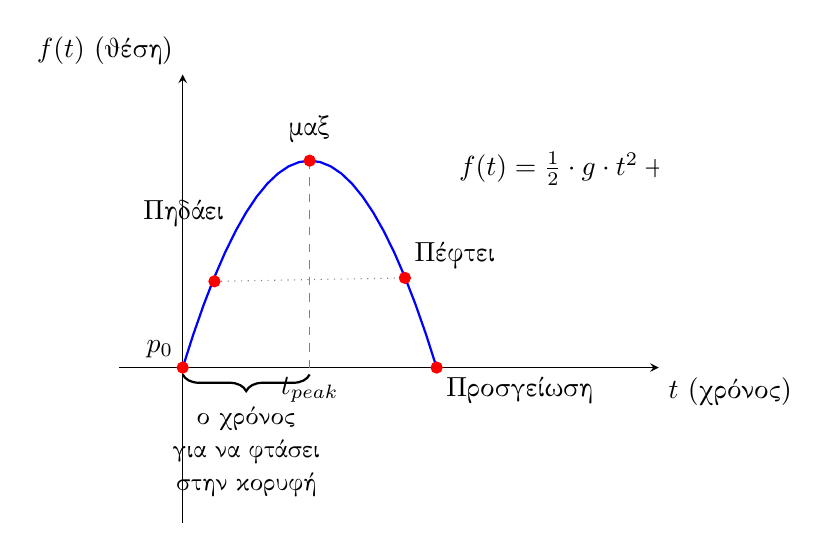
\begin{tikzpicture}
    \begin{axis}[
        axis lines = middle,
        xlabel = {$t$ (χρόνος)},
        ylabel = {$f(t)$ (θέση)},
        xtick=\empty,
        ytick=\empty,
        xmin=-1, xmax=7.5,
        ymin=-4.5, ymax=8.5,
        every axis x label/.style={at={(current axis.right of origin)},anchor=north west},
        every axis y label/.style={at={(current axis.above origin)},anchor=south east}
    ]
        \addplot[blue, thick, domain=0:4] {-1.5*x^2 + 6*x + 0};

        \draw[dashed, gray] (axis cs:2,6) -- (axis cs:2,0) node[below, black] {$t_{peak}$};
        \draw[dotted, gray] (axis cs:0.5,2.5) -- (axis cs:3.5,2.6);
        
        \draw[decorate, decoration={brace, amplitude=6pt, mirror}, thick]
             (axis cs:0,-0.2) -- (axis cs:2,-0.2)
             node[midway, below=8pt, black, align=center] {\small ο χρόνος\\ \small για να φτάσει\\ \small στην κορυφή};

        \addplot[only marks, mark=*, red] coordinates {
            (0,0)        
            (0.5,2.5)
            (2,6)        
            (3.5,2.6)
            (4,0)        
        };

        \node[above left] at (axis cs:0,0) {$p_0$};
        \node[above=3pt] at (axis cs:2,6) {max};
        \node[below right] at (axis cs:4,0) {Προσγείωση};
        
        \node[above left] at (axis cs:0.8, 3.8) {Πηδάει};
        \node[above right] at (axis cs:3.5, 2.6) {Πέφτει};
        
        \node[above right] at (axis cs:4.2, 5) {$f(t) = \frac{1}{2}\cdot g\cdot t^2 + v\cdot t + p_0$};
        
    \end{axis}
\end{tikzpicture}
\end{center}

\bigskip
\noindent\textbf{Πώς υπολογίζω το $v_0$ που χρειάζεται ο player για να φτάσει το max ύψος ($h$) σε $t_h$;}

\begin{align*}
    f'(t) &= g\cdot t + v_0, 
    \intertext{όπου $g$ η επιτάχυνση της βαρύτητας (η οποία είναι αρνητική).}
    \intertext{Όταν ο player φτάνει στο μέγιστο ύψος $h$, σταματάει να ανεβαίνει και ξεκινάει να πέφτει. Άρα η ταχύτητα $v$ στο $t = t_h$ είναι ίση με $0$:}
    f'(t_h) &= 0
    \intertext{Θέτοντας $t = t_h$ και $f'(t_h) = 0$ στη σχέση της ταχύτητας, έχουμε:}
    f'(t_h) &= g\cdot t_h + v_0 \\
    0 &= g\cdot t_h + v_0 \\
    &\implies v_0 = -g\cdot t_h
\end{align*}

\subsection*{Γράφημα Μεταβολής Ταχύτητας}

\begin{center}
\begin{tikzpicture}
    \begin{axis}[
        axis lines = middle,
        xlabel = {$t$ (χρόνος)},
        ylabel = {$f'(t)$ (ταχύτητα)},
        xtick=\empty,
        ytick=\empty,
        xmin=-1, xmax=6.5,
        ymin=-7.5, ymax=8.5,
        every axis x label/.style={at={(current axis.right of origin)},anchor=north west},
        every axis y label/.style={at={(current axis.above origin)},anchor=south east}
    ]
        \addplot[blue, thick, domain=0:4] {-3*x+6};
        \node[above right] at (axis cs:4.2,-3) {$f'(t) = g\cdot t +v_0$};
        \node[left] at (axis cs:0,6) {$v_0$};
        \node[left] at (axis cs:0,-6) {$-v_0$};
        
        \draw[dotted, gray, thick] (axis cs:4,0) node[above, black, yshift=2pt]{$2t_h$} -- (axis cs:4,-6);
        \draw[dotted, gray, thick] (axis cs:0,-6) -- (axis cs:4,-6);
    \end{axis}
\end{tikzpicture}
\end{center}

\bigskip
\textbf{Ποιά είναι η βαρύτητα όμως;}
\begin{itemize}
    \item \textbf{Αρχική θέση:} $p_0 = 0$
    \item \textbf{Ταχύτητα στην κορυφή:} $v(t_h) = 0 \implies v_0 = -g \cdot t_h$
    \item \textbf{Μέγιστο ύψος:} $f(t_h) = h$
\end{itemize}

\vspace{5pt}
Ξεκινάμε από τη γενική εξίσωση της θέσης:
\begin{align*}
    f(t) &= \frac{1}{2}\cdot g\cdot t^2 + v_0\cdot t + p_0 
    \intertext{Θέτουμε $t = t_h$, όπου η θέση είναι $f(t_h) = h$:}
    f(t_h) &= \frac{1}{2}\cdot g\cdot t_h^2 + v_0\cdot t_h + p_0 \\
    h &= \frac{1}{2}\cdot g\cdot t_h^2 + (-g \cdot t_h) \cdot t_h + 0 
    \intertext{Κάνουμε τις πράξεις:}
    h &= \frac{1}{2}\cdot g\cdot t_h^2 - g\cdot t_h^2 \\
    h &= -\frac{1}{2} g t_h^2 
    \intertext{Λύνουμε ως προς $g$:}
    g &= -\frac{2\cdot h}{t_h^2}
\end{align*}

\bigskip
\bigskip
Πάμε πίσω στο $v_0$ όπου έχουμε $v_0 = -g\cdot t_h$:
\begin{itemize}
    \item \textbf{Αρχική Ταχύτητα:} $v_0 = -g\cdot t_h$
    \item \textbf{Βαρύτητα:} $g = -\frac{2\cdot h}{t_h^2}$
\end{itemize}
Άρα:
\begin{align*}
    v_0 = -\left(\frac{-2\cdot h}{t_h^2}\right)\cdot t_h = \frac{2\cdot h}{t_h^2}\cdot t_h = \frac{2\cdot h}{t_h} 
\end{align*}
Επομένως:
\begin{equation*}
    v_0 = \frac{2\cdot h}{t_h} 
\end{equation*}

\vspace{20pt}
\hrule
\vspace{15pt}

Τα παραπάνω αφορούσαν αποκλειστικά το ύψος του άλματος. 
Πάμε τώρα να εξετάσουμε την \textbf{οριζόντια κίνηση} (απόσταση) του άλματος.

\vspace{10pt}
Είναι ιδιαίτερα χρήσιμο να ορίσουμε πόσο γρήγορα κινούμαστε δεξιά και αριστερά (\foreignlanguage{english}{lateral speed}). 
Για τον λόγο αυτόν, διατηρούμε την οριζόντια και την κάθετη ταχύτητα εντελώς \textbf{ξεχωριστά}.

\vspace{5pt}
\noindent\textbf{Γιατί συμβαίνει αυτό;} \\
Διότι αν ο παίχτης κινείται με ταχύτητα στον άξονα $x'x$ (οριζόντια) και πραγματοποιήσει άλμα (\foreignlanguage{english}{jump}), \textbf{δεν} επιθυμούμε να μηδενιστεί η οριζόντια ταχύτητά του και να κινηθεί αποκλειστικά κατακόρυφα. Αντιθέτως, απαιτείται η διατήρηση της ορμής του (\foreignlanguage{english}{momentum}).

\vspace{10pt}
Συνεπώς, καλούμαστε να ορίσουμε μια συνάρτηση η οποία λαμβάνει υπόψη της τρεις παραμέτρους:
\begin{enumerate}
    \item Την οριζόντια ταχύτητα στον άξονα $x'x$ (\foreignlanguage{english}{foot speed}).
    \item Τον χρόνο που απαιτείται για την επίτευξη του μέγιστου ύψους ($t_h$).
    \item Την οριζόντια απόσταση έως το σημείο $x_h$ (ή το συνολικό εύρος του άλματος).
\end{enumerate}

\vspace{5pt}
\noindent Η βέλτιστη πρακτική είναι μία από τις παραμέτρους αυτές να εξαρτάται από τις υπόλοιπες δύο. 
Η πιο απλή και λογική προσέγγιση είναι ο χρόνος να οριστεί ως εξαρτημένη μεταβλητή συναρτήσει των άλλων δύο παραμέτρων.
\bigskip
\noindent \\Ορίζουμε πλέον το $v_0$ και το $g$ ως συνάρτηση της οριζόντιας ταχύτητας (\textit{foot speed}) και της απόστασης έως το $x_h$:
\begin{equation*}
    t_h = \frac{x_h}{v_x}, \quad \text{όπου } v_x \text{ η ταχύτητα στον οριζόντιο άξονα (\textit{foot speed}).}
\end{equation*}

\vspace{5pt}
\noindent\textbf{Γιατί ισχύει αυτό;} \\
Στον οριζόντιο άξονα \textbf{δεν} υπάρχει επιτάχυνση (αγνοώντας την αντίσταση του αέρα), επομένως η κίνηση είναι ευθύγραμμη ομαλή. Άρα:
\begin{equation*}
    \Delta x = v_x \cdot t_h
\end{equation*}

Δεδομένου ότι $\Delta x = x_h - x_0$, αν θεωρήσουμε $x_0 = 0$, προκύπτει ότι $\Delta x = x_h$. Συνεπώς:
\begin{align*}
    x_h &= v_x \cdot t_h \\
    &\implies t_h = \frac{x_h}{v_x}
\end{align*}

\begin{center}
\begin{tikzpicture}
    \begin{axis}[
        axis lines = middle,
        xlabel = {$x$},
        ylabel = {$y$},
        xtick=\empty,
        ytick=\empty,
        xmin=-1, xmax=7.5,
        ymin=-4.5, ymax=8.5,
        every axis x label/.style={at={(current axis.right of origin)},anchor=north west},
        every axis y label/.style={at={(current axis.above origin)},anchor=south east}
    ]

        \addplot[blue, thick, domain=0:4] {-1.5*x^2 + 6*x + 0};

        \draw[dashed, gray] (axis cs:2,6) -- (axis cs:2,0) node[below, black] {$x_h$};
        \draw[dotted, black] (axis cs:0,6) node[above left, black]{$h$} -- (axis cs:2,6);
        
        \draw[-stealth, red, very thick] (axis cs:0.5, 0.5) -- (axis cs:2, 0.5) 
              node[midway, above] {$v_x$};

        \addplot[only marks, mark=*, red] coordinates {
            (2,6)
        };

        \node[above=3pt] at (axis cs:2,6) {max};

    \end{axis}
\end{tikzpicture}
\end{center}
\begin{itemize}
    \item \textbf{Αρχική ταχύτητα:} $v_0 = \frac{2 \cdot h}{t_h}$
    \item \textbf{Χρόνος για $f(x)=h$:} $t_h = \frac{x_h}{v_x}$
\end{itemize}

\begin{align*}
    v_0 &= \frac{2 \cdot h}{\frac{x_h}{v_x}} \iff v_0 = \frac{2 \cdot h \cdot v_x}{x_h} \\
    g &= -\frac{2 \cdot h}{t_h^2} \iff g = -\frac{2 \cdot h}{\left(\frac{x_h}{v_x}\right)^2} \iff \\
    g &= -\frac{2 \cdot h \cdot v_x^2}{x_h^2}
\end{align*}

\begin{center}
\begin{tikzpicture}
    \begin{axis}[
        axis lines = middle,
        xlabel = {$x$},
        ylabel = {$y$},
        xtick=\empty,
        ytick=\empty,
        xmin=-1.5, xmax=7.5,
        ymin=-0.5, ymax=8.5,
        every axis x label/.style={at={(current axis.right of origin)},anchor=north west},
        every axis y label/.style={at={(current axis.above origin)},anchor=south east}
    ]

        \addplot[blue, thick, domain=0:4] {-1.5*x^2 + 6*x + 0};

        \draw[dashed, gray] (axis cs:2,6) -- (axis cs:2,0) node[below, black] {$x_h$};
        \draw[dotted, black] (axis cs:0,6) node[above left, black]{$h$} -- (axis cs:2,6);
        
        \draw[-stealth, red, very thick] (axis cs:0.5, 0.5) -- (axis cs:2, 0.5) 
              node[midway, above] {$v_x$};
        \draw[-stealth, red, very thick] (axis cs:-0.5,6) -- (axis cs:-0.5,4) 
              node[midway, right] {$g$};
        \draw[-stealth, red, very thick] (axis cs:-0.9,4) -- (axis cs:-0.9,6)  
              node[midway, left] {$v_0$};
              
    \end{axis}
\end{tikzpicture}
\end{center}

\bigskip
\noindent Τα παραπάνω αντιστοιχούν στην απόλυτη φυσική πραγματικότητα. 
Ωστόσο, στο game development, συχνά επιλέγουμε να μην ακολουθήσουμε αυστηρά μια τέλεια μαθηματική
παραβολή, αλλά να την «τροποποιήσουμε» προκειμένου να πετύχουμε το επιθυμητό, ευχάριστο game feel και mechanics.
\subsection*{Fast Falling}

\begin{center}
\begin{tabular}{cc}
    \begin{tikzpicture}
        \begin{axis}[
            width=6.5cm, height=5.5cm,
            axis lines = middle,
            xlabel = {$t$},
            ylabel = {$f(t)$},
            xtick=\empty,
            ytick=\empty,
            xmin=-0.5, xmax=5,
            ymin=-1, ymax=8,
            every axis x label/.style={at={(current axis.right of origin)},anchor=north west},
            every axis y label/.style={at={(current axis.above origin)},anchor=south east}
        ]
            \addplot[gray!30, thick, domain=0:4] {-1.5*x^2 + 6*x + 0};

            \addplot[blue, thick, domain=0:2.83] {-3*x^2 + 6*x + 0}; % Άνοδος
            \addplot[red, thick, domain=2.83:3.46] {-3*x^2 + 6*x + 0};  % Πτώση

            \draw[dashed, gray] (axis cs:1,3) -- (axis cs:1,0);
            \draw[dashed, gray] (axis cs:0,3) -- (axis cs:1,3);

        \end{axis}
    \end{tikzpicture}
    &
    \begin{tikzpicture}
        \begin{axis}[
            width=6.5cm, height=5.5cm,
            axis lines = middle,
            xlabel = {$t$},
            ylabel = {$v(t)$},
            xtick=\empty,
            ytick=\empty,
            xmin=-0.5, xmax=5,
            ymin=-6, ymax=8,
            every axis x label/.style={at={(current axis.right of origin)},anchor=north west},
            every axis y label/.style={at={(current axis.above origin)},anchor=south east}
        ]
            \addplot[blue, thick, domain=0:2] {-3*x + 6};
            
            \addplot[red, thick, domain=2:3.5] {-5*x + 10};

            \draw[dashed, gray] (axis cs:2,0) -- (axis cs:2,-2);
            \draw[thin, gray] (axis cs:0,-2) -- (axis cs:2,-2);

        \end{axis}
    \end{tikzpicture}
    \\
    {\small \textit{Position}} & {\small \textit{Velocity / Acceleration}}
\end{tabular}
\end{center}
\subsection*{Variable Height Jumping}

\begin{center}
\begin{tabular}{cc}
    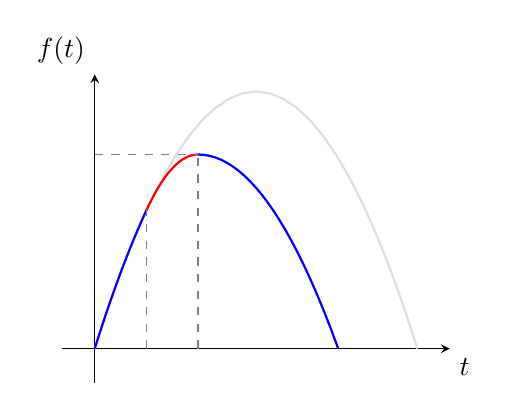
\begin{tikzpicture}
        \begin{axis}[
            width=6.5cm, height=5.5cm,
            axis lines = middle,
            xlabel = {$t$},
            ylabel = {$f(t)$},
            xtick=\empty,
            ytick=\empty,
            xmin=-0.5, xmax=5.5,
            ymin=-1, ymax=8,
            every axis x label/.style={at={(current axis.right of origin)},anchor=north west},
            every axis y label/.style={at={(current axis.above origin)},anchor=south east}
        ]
            \addplot[gray!25, thick, domain=0:5] {-1.2*x^2 + 6*x};

            \addplot[blue, thick, domain=0:0.8] {-1.2*x^2 + 6*x}; 
            
            \addplot[red, thick, domain=0.8:1.6] {-2.55*(x-0.8)^2 + 4.08*(x-0.8) + 4.032}; 
            
            \addplot[blue, thick, domain=1.6:3.77] {-1.2*(x-1.6)^2 + 5.664}; 

            \draw[dashed, gray] (axis cs:0.8,0) -- (axis cs:0.8,4.032);
            \draw[dashed, gray] (axis cs:1.6,0) -- (axis cs:1.6,5.664);
            \draw[dashed, gray] (axis cs:0,5.664) -- (axis cs:1.6,5.664);

        \end{axis}
    \end{tikzpicture}
    &
    \begin{tikzpicture}
        \begin{axis}[
            width=6.5cm, height=5.5cm,
            axis lines = middle,
            xlabel = {$t$},
            ylabel = {$v(t)$},
            xtick=\empty,
            ytick=\empty,
            xmin=-0.5, xmax=5.5,
            ymin=-6, ymax=8,
            every axis x label/.style={at={(current axis.right of origin)},anchor=north west},
            every axis y label/.style={at={(current axis.above origin)},anchor=south east}
        ]
            \addplot[blue, thick, domain=0:0.8] {-2.4*x + 6};
            
            \addplot[red, thick, domain=0.8:1.6] {-5.1*(x-0.8) + 4.08};
            
            \addplot[blue, thick, domain=1.6:3.77] {-2.4*(x-1.6)};

            \draw[dashed, gray] (axis cs:0.8,0) -- (axis cs:0.8,-2.4);
            \draw[dashed, gray] (axis cs:1.6,0) -- (axis cs:1.6,-5.1);

            \draw[blue, thick] (axis cs:0,-2.4) -- (axis cs:0.8,-2.4);
            \draw[red, thick] (axis cs:0.8,-5.1) -- (axis cs:1.6,-5.1);
            \draw[blue, thick] (axis cs:1.6,-2.4) -- (axis cs:3.77,-2.4);

        \end{axis}
    \end{tikzpicture}
    \\
    {\small \textit{Position}} & {\small \textit{Velocity / Acceleration}}
\end{tabular}
\end{center}
\subsection*{Double Jumping}

\begin{center}
\begin{tabular}{cc}
    \begin{tikzpicture}
        \begin{axis}[
            width=6.5cm, height=5.5cm,
            axis lines = middle,
            xlabel = {$t$},
            ylabel = {$f(t)$},
            xtick=\empty,
            ytick=\empty,
            xmin=-0.5, xmax=8,
            ymin=-1, ymax=10,
            every axis x label/.style={at={(current axis.right of origin)},anchor=north west},
            every axis y label/.style={at={(current axis.above origin)},anchor=south east}
        ]
            \addplot[blue, thick, domain=0:2.5] {-1.2*x^2 + 4.8*x}; 
            
            \addplot[gray!25, thick, domain=2.5:4] {-1.2*x^2 + 4.8*x};

            \addplot[red, thick, domain=2.5:7.33] {-1.2*(x-2.5)^2 + 4.8*(x-2.5) + 4.5}; 

            \draw[dashed, gray] (axis cs:2,4.8) -- (axis cs:2,0); % peak 1
            \draw[dashed, gray] (axis cs:2.5,0) -- (axis cs:2.5,4.5); % trigger point
            \draw[dashed, gray] (axis cs:2.5,4.5) -- (axis cs:4.5,4.5); % reference line
            \draw[dashed, gray] (axis cs:4.5,4.5) -- (axis cs:4.5,9.3); % peak 2

        \end{axis}
    \end{tikzpicture}
    &
    \begin{tikzpicture}
        \begin{axis}[
            width=6.5cm, height=5.5cm,
            axis lines = middle,
            xlabel = {$t$},
            ylabel = {$v(t)$},
            xtick=\empty,
            ytick=\empty,
            xmin=-0.5, xmax=8,
            ymin=-7, ymax=8,
            every axis x label/.style={at={(current axis.right of origin)},anchor=north west},
            every axis y label/.style={at={(current axis.above origin)},anchor=south east}
        ]
            \addplot[blue, thick, domain=0:2.5] {-2.4*x + 4.8};
            
            \addplot[red, thick, domain=2.5:7.33] {-2.4*(x-2.5) + 4.8};

            \draw[gray!50, thin] (axis cs:2.5,-5) -- (axis cs:2.5,7);

            \draw[blue, thick] (axis cs:0,-2.4) -- (axis cs:2.5,-2.4);
            \draw[red, thick] (axis cs:2.5,-3.5) -- (axis cs:7.33,-3.5);

        \end{axis}
    \end{tikzpicture}
    \\
    {\small \textit{Position}} & {\small \textit{Velocity / Acceleration}}
\end{tabular}
\end{center}
\subsection*{Integration}

Για την ενημέρωση της κίνησης του παίκτη,από την κατάσταση \textit{current state} στην \textit{feature state} σε κάθε χρονικό βήμα $\Delta t$, απαιτείται ο υπολογισμός της νέας θέσης και ταχύτητας. 

\vspace{10pt}
\noindent\textbf{1. Μέθοδος Euler (Euler Integration)}
\begin{align*}
    \text{\textbf{Pseudocode:}} \quad & \mathtt{pos} \mathrel{+}= \mathtt{vel} \cdot \Delta t \\
    & \mathtt{vel} \mathrel{+}= \mathtt{acc} \cdot \Delta t
\end{align*}
\textbf{Πλεονεκτήματα / Μειονεκτήματα:} Είναι η απλούστερη μέθοδος υλοποίησης, αλλά παρουσιάζει μεγάλη αστάθεια και συσσωρεύει σφάλματα (είναι μη αξιόπιστη για ακριβή φυσική).

\vspace{10pt}
\noindent\textbf{2. Μέθοδος Runge-Kutta 4ης Τάξης (RK4)} \\
Πρόκειται για μια ιδιαίτερα ακριβή αλλά αρκετά σύνθετη μέθοδο υπολογισμού. Προσφέρει την υψηλότερη πιστότητα, αλλά απαιτεί περισσότερους υπολογιστικούς πόρους.

\vspace{10pt}
\noindent\textbf{3. Μέθοδος Velocity Verlet}
\begin{align*}
    \text{\textbf{Pseudocode:}} \quad & \mathtt{pos} \mathrel{+}= \mathtt{vel} \cdot \Delta t + \frac{1}{2} \cdot \mathtt{acc} \cdot \Delta t^2 \\
    & \mathtt{new\_acc} = f(\mathtt{pos}) \\
    & \mathtt{vel} \mathrel{+}= \frac{1}{2} \cdot (\mathtt{acc} + \mathtt{new\_acc}) \cdot \Delta t \\
    & \mathtt{acc} = \mathtt{new\_acc}
\end{align*}

\vspace{5pt}
\noindent Επειδή στη δική μας περίπτωση η επιτάχυνση (βαρύτητα $g$) είναι σχεδόν πάντα **σταθερή** ($\mathtt{acc} = \mathtt{new\_acc}$), ο αλγόριθμος απλοποιείται ως εξής:

\begin{align*}
    \text{\textbf{Απλοποιημένος Pseudocode:}} \quad & \mathtt{pos} \mathrel{+}= \mathtt{vel} \cdot \Delta t + \frac{1}{2} \cdot \mathtt{acc} \cdot \Delta t^2 \\
    & \mathtt{vel} \mathrel{+}= \mathtt{acc} \cdot \Delta t
\end{align*}
\end{document}